\chapter{\label{sec:conclusion} Conclusions}

In this thesis, we have presented a chain of techniques that allow us to efficiently animate densely scanned models of physical objects. By creating a layered model consisting of a skeleton structure, a control mesh and a detailed mesh, we make it much easier for animators to use these dense models. 

We have defined a method for the animation of simple meshes based on a skeleton structure, which requires minimal operator intervention, other than the colocation of the skeleton and the mesh to be animated. This aspect of the layered model can be used at the animation planning stage in order to enable an animator to prepare animations of complex surfaces in real time. This control mesh animation scheme was implemented in VRML, using methods which have since been integrated into proposed international standards for human body animation.

We then presented a method of automatically mapping a detailed scanned surface layer to this control mesh. This mapping allows smooth animation of the dense surface to be driven by animation of the control mesh, allowing this control layer to be used for interactive applications, while the animated detail layer can be automatically rebuilt for offline rendering.

We also presented an alternative representation of the detail layer as a displacement map defined over the control mesh. The representation allows animation and reconstruction of the detail layer at arbitrary levels of detail, allowing rendering of the detail layer to be performed at any resolution and speed as defined by the animator. Displacement mapped models also have applications for simple mesh editing and efficient compression of dense data.

We assert that this layered framework provides a useful tool for the animation of such dense data, allowing animators to utilise objects from the real world directly in their work with the minimum of manual intervention. Displacement mapping techniques also allow the use of highly-detailed models in interactive applications, such as games.

\section{\label{sec:conclusion:dispsubdiv}Displaced Subdivision Surfaces}

As noted in section \ref{sec:litreview:modeling:detail}, a similar method of representing detailed surfaces was proposed by \citet{Lee00}, in the form of Displaced Subdivision Surfaces. Both this method and our own were developed concurrently, and are similar in many ways. Lee et al. represent the detailed surface as a displacement map, but instead of basing the map on a polygonal control mesh as we do, they use a Loop subdivision surface \cite{Loop94} as the base domain. This has some advantages, but also imposes some limitations on their method.

\begin{figure}
\begin{center}
\begin{tabular}{cc}
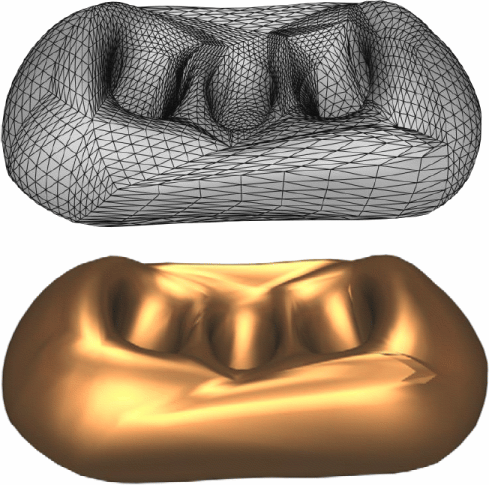
\includegraphics[width=5cm]{../images/lee_poly} &
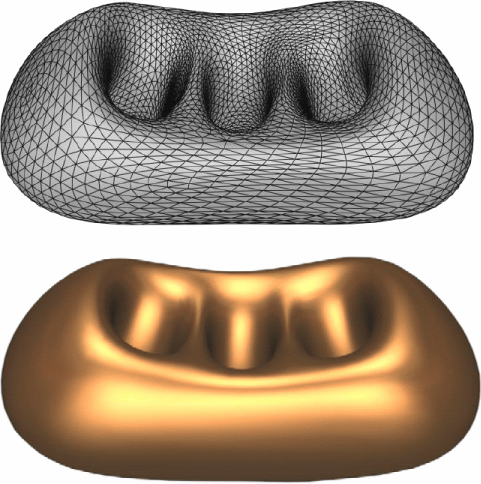
\includegraphics[width=5cm]{../images/lee_subdiv} \\
{\it(a)} & {\it(b)}
\end{tabular}
\caption[Displaced Subdivision Surfaces]{\label{fig:dispsubdiv} Displaced Subdivision Surfaces. The images above compare displacement map animation using (a) polyhedral and (b) smooth base domains. The reconstruction based on the polyhedral base domain is distorted. However, this is due mainly to the fact that the polyhedral domain is unsuitable for the animation being performed. Images taken from \cite{Lee00}.}
\end{center}
\end{figure}
Firstly, Lee's use of a smooth base domain allows smoother animation of the displaced surface. Our polygonal control mesh is piecewise linear, with only C0 continuity. The use of the interpolated normals counteracts this to an extent, but does not increase the mathematical smoothness of the surface. Lee's smooth base domain is C1 continuous at all points, enabling smoother animation of the displaced surface. In \cite{Lee00}, Lee compares displacement map animation based on both a polygonal control mesh and the Loop subdivision surface generated from it, pointing out that the polygonal version suffers from large distortions during animation. These distortions are shown in figure \ref{fig:dispsubdiv}. However, most of these distortions are caused by the fact that the control mesh used is automatically generated from the dense surface, which often results in a control mesh unsuitable for animation. As discussed above, if a polygonal control mesh is designed by hand for animation, good results can be obtained without the need for a smooth domain surface, simplifying the method.

Secondly, both Lee's method and our own generate a mapping between two similar meshes, in order to convert a detailed surface into a displacement map based on a simpler control surface. Lee calculates this mapping as part of the MAPS algorithm \cite{Lee99} which also generates the control surface automatically as part of the same process. This means that Lee's method can only be used with such automatically generated control surfaces, which as mentioned above may be unsuitable for animation themselves. A skilled animator cannot use a pre-existing stock model as the control surface, nor use his expertise to design a suitable control surface manually. Our method defines a general method of calculating a mapping between pairs of similar meshes, and thus allows more flexibility and control.

The final major difference between the two methods is that when the displacement map is created, Lee uses a raycasting method as described in section \ref{sec:dispmapcreation:raycasting}, which explicitly calculates the displacement value of each pixel in the displacement map by measuring the distance to the detail layer. Conversely, our method draws triangles into the displacement map based on the existing detail layer mapping results. Lee's method involves a search of potentially every triangle in the detail layer for each pixel in the displacement map, while our method contains no such searching, and therefore should be more efficient.

In conclusion, the two approaches perform very similar functions, but have a few fundamental differences. Lee takes a fully automatic approach which gives mathematically smooth animation, while we present a more flexible and efficient method which requires expert input to get the best results. However, professional animators usually prefer semi-manual approaches to fully automatic, so we expect that our method will be more useful for practical animation use.

\section{\label{sec:conclusion:future}Future Work}

There are many ways in which the layered animation system can be extended and improved, for instance in the area of skeletal animation as discussed in section \ref{sec:skeletalanim:conclusion:future}.  A number of these improvements concern problems of user interaction and feedback. For example, as discussed in section \ref{sec:scandata:creation:control:semiautomatic}, a semi-automatic approach may be the best solution to the creation of the control layer, allowing an animator to define a suitable control layer while preserving constraints such as injectivity for displacement mapping. Such a system could also alert the animator to collapsing normal volumes (discussed in section \ref{sec:scandata:normalvolume:collapse}) during the creation process, and also during animation. The user could then adjust the control layer to avoid collapses and ensure that good results are obtained.

As discussed in section \ref{sec:dispmapanim:editing}, displacement maps lend themselves to simple editing in two dimensions. However, it can be difficult to gauge the effects of a 2D displacement map edit on the 3D surface. Therefore, some kind of instant feedback system would be useful, where the user can see the change in the surface as the map is edited in 2D. This would require very fast recalculation and display of the displacement mapped model, so would require a method of performing the reconstruction process in real time.

\subsection{\label{sec:conclusion:future:realtime}Realtime Displacement Mapping}

By using the displacement mapping techniques we have proposed, and by taking advantage of recent advances in rendering technology, it is possible to render dense scanned meshes (or a close approximation thereof) in real time, for use in interactive graphics systems such as games. Indeed, the latest DirectX 9 API from \citet{DirectX9} provides direct support for displacement mapped models, and it is likely that OpenGL \cite{OpenGL} will follow suit in the near future.

\subsubsection{\label{sec:conclusion:future:realtime:shaders}Shaders}

The latest consumer graphics hardware has disposed of the traditional fixed-function rendering pipeline that has dominated the industry until recently. Instead, modern graphics chipsets include the capability to reprogram various parts of the pipeline \cite{Lindholm01}, using short programs known as {\it shaders}, which are loaded onto the card for execution during rendering \cite{Proudfoot01}. Shaders have been used for many years in high-end graphics languages such as Pixar's RenderMan \cite{Apodaca99}, which are traditionally used on large rendering farms for film production. They fall into two main classes, {\it vertex} and {\it fragment} shaders. Both are normally programmed in assembly language, though higher level languages have recently been introduced to ease the programming process \cite{Mark03}.

Vertex shaders replace the {\it Transform and Lighting} stage of the fixed-function pipeline, and operate on single vertices. They can modify the position, lighting, texture information and other properties of these vertices before they are passed into the later stages of the pipeline. While current vertex shaders do not allow access to actual texture data, forthcoming versions will have this capability, which will allow them to perform the post-subdivision point reconstruction step of displacement map rendering as described in section \ref{sec:dispmapanim:reconstruction:sampling}. The vertex shader will carry out sampling of the displacement map, as well as the various vector interpolation operations required to rebuild the correct 3D surface point, all using dedicated hardware. A vertex shader could also implement the skeletal animation component of the system, further easing CPU load.

Fragment shaders operate at a later stage in the pipeline, where they determine the colour of a single fragment (which can be thought of as a pixel) on the screen. While fragment shaders can not modify geometry, they can be used to implement algorithms such as bump mapping. 

In a system designed to render detailed models in real time, the main CPU would perform only the subdivision step of the displacement map rendering. A vertex program would then perform the vertex rebuilding for each subdivided vertex, and a fragment program could display a bump map generated from the displacement map. This would give the appearance of a highly detailed model, rendered in real time.

\subsubsection{\label{sec:conclusion:future:realtime:subdivision}Subdivision Optimisation}

It is possible to speed up the rendering process described above by precalculating the levels of subdivision for the control mesh. In the games industry in particular, precalculation is extensively used to avoid expensive computation, and in an environment where speed is more important than memory usage, this is a valid and successful strategy.

It is possible that even the subdivision stage of displacement map rendering could be performed on graphics hardware, eliminating the need for such optimisations. \citet{Vlachos01} describe a system which has already been implemented in the {\it Truform} feature on ATI  graphics hardware \cite{ATI01}, which is capable of subdividing and smoothing a triangle mesh without any intervention on the part of the programmer. The system uses spare GPU power to subdivide models as much as possible without affecting the frame rate of the result, and could easily be adapted to perform displacement map rendering purely in hardware.

\section{\label{sec:conclusion:fin}Epilogue}

Graphics technology advances at an ever-increasing rate, and techniques that seemed far from real-world application five years ago are about to become commonplace. The original vision of this project, the realtime animation of dense datasets, may not be an issue for much longer, as the average PC can now render such models in realtime with ease. With our layered displacement mapping techniques however, we believe we have created a method of working with such dense data that will greatly ease the task of those who must create the content for a new world of ubiquitous 3D.
